% Chapter Template

\chapter{Introducción} % Main chapter title

\section{Antecedentes}

Desde su formulación inicial en la década de 1920, se hizo evidente que la Mecánica Cuántica es una teoría radicalmente distinta al resto de la Física conocida hasta ese entonces. Uno de los ejemplos más sorprendentes de esto es el efecto túnel o tunelamiento. Descubierto inicialmente por George Gamow en 1928 para explicar el decaimiento alfa \cite{gamow1928quantum}, este fenómeno permite a una partícula atravesar una barrera de potencial, a pesar de que no pueda hacerlo clásicamente por no contar con la energía suficiente. %Desde su descubrimiento, ha encontrado un gran número de aplicaciones en las diversas áreas de la física, constituyendo una de las piedras angulares en la construcción de la ciencia y tecnología modernas.

Una consecuencia importante del tunelamiento en la Teoría Cuántica de Campos es el decaimiento del falso vacío, tema a tratar en este trabajo. En este caso, la partícula atraviesa la barrera de potencial para decaer finalmente al estado de mínima energía. El estudio de este fenómeno se inicio con el trabajo de Voloshin et. al. \cite{Kobzarev:1974cp}, el cual fue extendido y desarrollado en detalle por Coleman y Callan a fines de los años 70 \cite{coleman1977fate, callan1977fate}. Posteriormente, Coleman y DeLuccia incluyeron los efectos de la gravedad en su teoría \cite{coleman1980gravitational} y basándose en esta, Guth propuso un modelo inflacionario del universo que resolvía el enigma de cómo podría haberse expandido extremadamente rápido para luego acercarse a un estado plano \cite{guth1981inflationary}. Muchos otros se basaron en este trabajo para encontrar nuevas clases de soluciones al problema, siendo algunos ejemplos notables los de Hawking y Moss \cite{hawking1982supercooled}, Hawking y Turok \cite{hawking1998open}, y Hackworth y Weinberg \cite{hackworth2005oscillating}.

El decaimiento del falso vacío encuentra importantes aplicaciones en diversas áreas de la Física, principalmente en la física de altas energías. En la cosmología, cumple un papel esencial en diversos modelos de inflación en el Universo temprano \cite{guth2007eternal}. El hecho de que el Universo tenga un tiempo de vida finita, da pie a la posibilidad de que al momento de expandirse y enfriarse, se haya establecido en el falso vacío \cite{coleman1977fate}.   Por otro lado, las mediciones más recientes del vacío electrodébil, relacionado con el potencial de Higgs, parecen indicar que este es metaestable antes que estable \cite{bass2021higgs}. A su vez, los últimos cálculos realizados  tiempo de vida sugieren que es mayor que la edad del Universo, reforzando el escenario metaestable \cite{andreassen2018scale}. Por último, el decaimiento del falso vacío también tiene aplicaciones en la teoría de cuerdas, la física estadística y la física de la materia condensada por ejemplo, en superconductividad \cite{paranjape2017theory}   %, desde la física de partículas hasta la cosmología. 
%El decaimiento del vacío, es decir, la transición de fase cuántica de primer orden fuera de un estado de falso vacío metaestable, juega un papel importante en los modelos actuales del universo temprano. Esto incluye las teorías de la inflación eterna del falso vacío \cite{guth2007eternal}), transiciones de fase de ruptura de simetría en las teorías de gran unificación \cite{guth1981cosmological}, y tal vez incluso en el Modelo Estándar de la física de partículas \cite{ellis2009probable}. La dinámica de estas transiciones tiene implicaciones para la solución del problema de la constante cosmológica, la observabilidad del falso vacio, la inflación eterna en el multiverso \cite{aguirre2007towards}, el futuro del vacío de Higgs \cite{feeney2011first} y las señales de ondas gravitacionales primordiales \cite{kosowsky1992gravitational} dentro de la banda de futuros experimentos como la Antena espacial de interferómetro láser (LISA) \cite{axen2018multiwavelength}.
%Recientemente, fueron propuestos pruebas de laboratorio utilizando como modelo experimental un gas de Bose ultrafrío \cite{fialko2015fate}. Más específicamente, se utiliza el condensado de Bose-Einstein (BEC) de dos componentes atómicos ultrafrío como simulador cuántico para generar un falso vacío relativista en decaimiento. Las simulaciones numéricas demuestran la formación espontánea de burbujas del verdadero vacío con parámetros y escalas de tiempo realistas \cite{billam2019simulating}.

El decaimiento del falso vacío puede verse afectado por efectos gravitacionales. Por ejemplo, los agujeros negros pueden actuar como centros de nucleación incrementando la tasa de decaimiento. De igual manera, puede ser una fuente de ondas gravitacionales y efectos más allá del Modelo Estándar de partículas elementales \cite{Ai:2019dqr}. 

               .

\section{Objetivo}

%\colorbox{yellow}{revisar}
Consideremos un potencial como el de la figura \ref{fig:potencial} que posee dos mínimos distintos, uno mayor que otro. Clásicamente, ambos puntos son estables. Sin embargo, esta no es la situación a nivel cuántico. Debido al efecto túnel, existe la posibilidad de que una partícula que se encuentre inicialmente en $x_+$, atraviese la barrera %reapareciendo por $x_0$                                                            
al estado de menor energía del sistema. Es por esto que a $x_+$ se le denomina como falso vacío y a este proceso como decaimiento del falso vacío.
A lo largo del trabajo tomaremos la figura \ref{fig:potencial} como nuestro potencial de referencia. % al momento de realizar los cálculos. 

\begin{figure}[t]
	\centering
	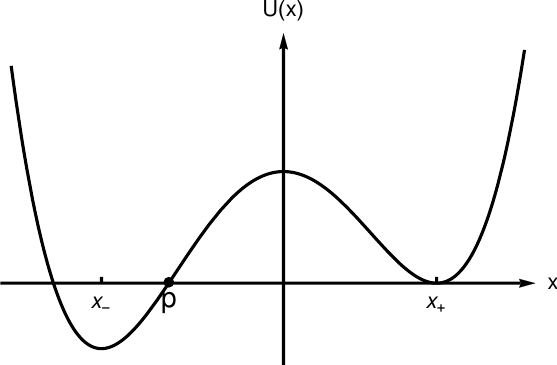
\includegraphics[scale = 0.4]{../FIGURAS/potencial}
	\caption{Potencial con un falso vacío en $x_+$ \cite{Ai:2019dqr}.}
	\label{fig:potencial}
\end{figure}

%\section{Objetivo}

El objetivo principal del presente trabajo de investigación es el cálculo de la tasa de decaimiento del falso vacío $\Gamma$ a primer orden en $\hbar$. 
%para el estado metaestable de menor energía
Inicialmente se llevará a cabo en la Mecánica Cuántica haciendo uso de la integral de camino euclideana y la aproximación del punto estacionario siguiendo el formalismo planteado originalmente por Coleman y Callan \cite{coleman1977fate, callan1977fate}. %Primero se estudiará este fenómeno en la Mecánica Cuántica y luego en la Teoría Cuántica de Campos del campo escalar. 
Posteriormente el mismo será extendido a la Teoría Cuántica de Campos del campo escalar donde además se analizará  la formación de las burbujas de verdadero vacío y su evolución espaciotemporal haciendo uso de la aproximación de la pared delgada. 




%\begin{figure}[h]
%	\centering
%	\begin{tikzpicture}[scale = 2]
%	
%	\draw[<->] (-2, 0) -- (2, 0) node[anchor = west] {$x$}; 
%	\draw[<->] (0,-1) -- (0,2) node[anchor = south] {$V(x)$};
%	
%	\draw[line width = 0.5mm, color = blue, domain = -1.5:1.5, smooth] plot(\x, {((\x - 1)^2)*((\x + 1)^2) - 0.2*(\x + 1)});
%	
%	\node[anchor = north] at (-1, 0) (a) {$a$};
%	\draw (-1,-0.05) -- (-1,0.05);
%	
%	\node[anchor = north] at (-1, 0) (a) {$a$};
%	\draw (-1,-0.05) -- (-1,0.05);
%	
%	\node[anchor = southleine] at (1, 0) (b) {$b$};
%	\draw (1,-0.05) -- (1,0.05);
%	\end{tikzpicture}
%	%\caption{Potencial para el estudio numérico del decaimiento del falso vacío. Cuenta con una región de falso (FV) y verdadero vacío (R), separados por una barrera (B) \cite{Masoumi:2015psa}.}
%	%\label{fig:potencial_numerico} 
%\end{figure}







